\section{Ejercicio 5: Comparación}

  % \begin{figure}[ht]
  %   \begin{center}
  %     \includegraphics[width=0.5\columnwidth]{imagenes/pacman.png}
  %     \caption{Perdidos y con poca fuerza}
  %   \end{center}
  % \end{figure}

    % 1. Describir detalladamente el problema a resolver dando ejemplos del mismo y sus soluciones.
    \subsection{Hipótesis}
        Para realizar un análisis exhaustivo y poder realizar conclusiones generales sobre las distintas implementaciones de nuestro problema, se pidió por último hacer una experimentacion acorde para poder compararlas, en donde se usaron las mejores configuraciones halladas (particularmente para los ejercicios 3 y 4) en cuanto a calidad de la solución.

        Se realizaron dos experimentos. El primero consistió en un análisis y comparación de la calidad de los resultados obtenidos y del tiempo de procesamiento que demandaron todas las implementaciones realizadas. El segundo experimento consistió en el mismo análisis y comparación pero sólo de las implementaciones no exactas (ejercicios 2, 3 y 4). Para ambos experimentos se utilizó una configuración considerada "buena" en cuanto a calidad de solución para las heurísticas (Vecindario A, RCL = 2, criterio de GRASP de 30 iteraciones en las cuales no se haya encontrado ninguna solución mejor).
        Las instancias fueron generadas de manera aleatoria sin repetir cantidad de estaciones totales (gimnasios + pokeparadas), y se intentó acercarse a que haya al menos una posible solución colocando en cada instancia la cantidad de pokeparadas igual a $\sum_{g \in Gimnasios} pociones(g)$, con una cantidad random entre 1 y 10 pociones por gimnasio para el primer experimento y entre 1 y 50 para el segundo, y un tamaño de mochila igual a 3 veces la cantidad de pokeparadas de manera que alcance para guardar todas las pociones de todas las pokeparadas. Las ubicaciones de las pokeparadas y los gimnasios también fueron seleccionadas de manera random con cada par $(x,y)$ $x$ e $y$ entre 1 y 1000. Para el primer experimento se utilizaron 15 instancias aleatorias, en la cual la cantidad de gimnasios se varió entre 1 y 7 y la suma de gimnasios más pokeparadas sea menor o igual a 16, mientras que para el segundo experimento se realizaron 99 instancias donde la cantidad de gimnasios varió entre 1 y 50 y la suma de gimnasios más pokeparadas sea menor o igual a 100.

        Teniendo en cuenta la experimentación realizada a lo largo de este trabajo, esperábamos que la metaheruística tenga mejores resultados que la heurística greedy y la búsqueda local, pero que no haya mucha diferencia temporal entre ellas incluso para instancias grandes y a pesar de la cota de complejidad propuesta para el ejercicio 3.

    \subsection{Experimento 1}
        En este experimento se utilizaron instancias de hasta 16 estaciones para que los tiempos y soluciones puedan ser comparados con el algoritmo de Backtracking.
        En una comparación entre los 4 algoritmos incluyendo las 16 instancias, construimos la siguiente tabla con estadísticas al respecto. En la misma, el promedio realizado es sobre los resultados de las 16 instancias evaluadas 30 veces cada una.

\begin{flushleft}
\begin{tabular}{l | rrrrrrrrr}
\toprule
{} &       Tiempo en ns  &       Gyms &  Pokeparadas &     Mochila &    Distancia &  Estaciones visitadas &  Nro. Ej \\
\midrule
promedio  &  6,104684e+09 &   3,25     &    6,25     &   16,4375   &  1811,2025   &            9,0625   &      1 \\
promedio  &  54172,085595 &   3,25     &    6,25     &   16,4375   &  2464,306785 &            9,298539 &      2 \\
promedio  &  60037,843750 &   3,25     &    6,25     &   16,4375   &  2452,986250 &            9,298539 &      3 \\
promedio  &  6,175643e+07 &   3.25     &    6.25     &   16.4375   &  2202.168813 &            9.091667 &      4 \\
\hline
min   &  326          &   1        &    1        &   0         &  0           &            1        &      1 \\
min   &  284          &   1        &    1        &   0         &  0           &            1        &      2 \\
min   &  978          &   1        &    1        &   0         &  0           &            1        &      3 \\
min   &  7.925460e+06 &   1        &    1        &   0         &  0           &            1        &      4 \\
\hline
max   &  6,290560e+10 &   6        &    11       &   31        &  3041,12     &            16       &      1 \\
max   &  314883       &   6        &    11       &   31        &  3922,82     &            17       &      2 \\
max   &  531943       &   6        &    11       &   31        &  3922.82     &            17       &      3 \\
max   &  1.256230e+08 &   6        &    11       &   31        &  4135.69     &            17       &      4 \\
\bottomrule
\end{tabular}      
\end{flushleft}

      En cada fila se calculó el promedio, mínimo y máximo de las variables estudiadas de manera independiente para cada ejercicio. El número perteneciente a la columna de \emph{Estaciones visitadas} corresponde al valor de estaciones visitadas de la solución obtenida.

      Observamos que en cuanto a los promedios el más cercano al ejercicio 1 es, como esperabamos, el ejercicio 4. Particularmente en el número de estaciones visitadas, la distancia recorrida y el tiempo. Pero además esto nos muestra que a pesar de dar una solución cercana, el tiempo que toma es mucho mayor al de los otros dos ejercicios, cosa que nos sorprendió al momento del análisis de los resultados contradiciendo nuestra hipótesis.

      En cuanto a los mínimos obtenidos cabe destacar que es normal que el ejercicio 4 tome más tiempo que los demás, puesto que de por sí tiene la configuración de realizar 30 iteraciones que no den resultados mejores.

      Por último, el máximo del ejercicio 4 fue uno de los peores en cuanto a calidad de la solución y entendemos que esto se debe a la aleatoriedad que tiene en su implementación. Los máximos tiempos que tomaron los ejercicios 2 y 3 son evidentemente los menores, lo cual era lo esperado. El ejercicio 4 si bien toma mucho más tiempo que los anteriores dos, sigue siendo aproximadamente 100 veces más rápido que el ejercicio 1.

      Para mostrar cómo evoluciona el tiempo en funcion de la cantidad de estaciones de cada algoritmo, plasmamos los resultados obtenidos en este experimento en este gráfico:

\begin{figure}[H]
    \begin{center}
      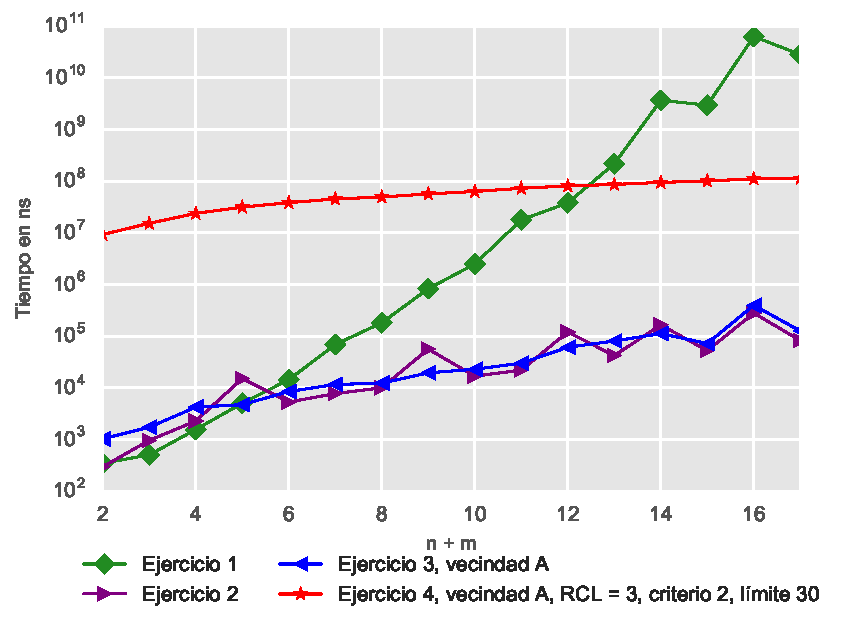
\includegraphics[\columnwidth]{imagenes/tiempo_16_buena_distancia.pdf}
      \caption{}
    \end{center}
\end{figure}

      Observamos que como mostraba la tabla, los ejercicios 2 y 3 se mantienen cercanos en cuanto a tiempo. Por otro lado, el ejercicio 1 crece exponencialmente y el ejercicio 4 se mantiene entre $10^7$ y $10^8$. Notamos cómo a partir de las 12 estaciones, la implementación de GRASP toma menos tiempo que la implementación de backtracking por lo que si GRASP efectivamente diera una buena solución y estuvieramos dispuestos a renunciar a efectividad sobre tiempo, entonces sería una buena opción para instancias grandes.

      Para analizar la calidad de la solución con un poco más de detalle generamos el siguiente gráfico de barras que muestra la distancia recorrida en función del tamaño de la instancia para cada implementación.

\begin{figure}[H]
    \begin{center}
      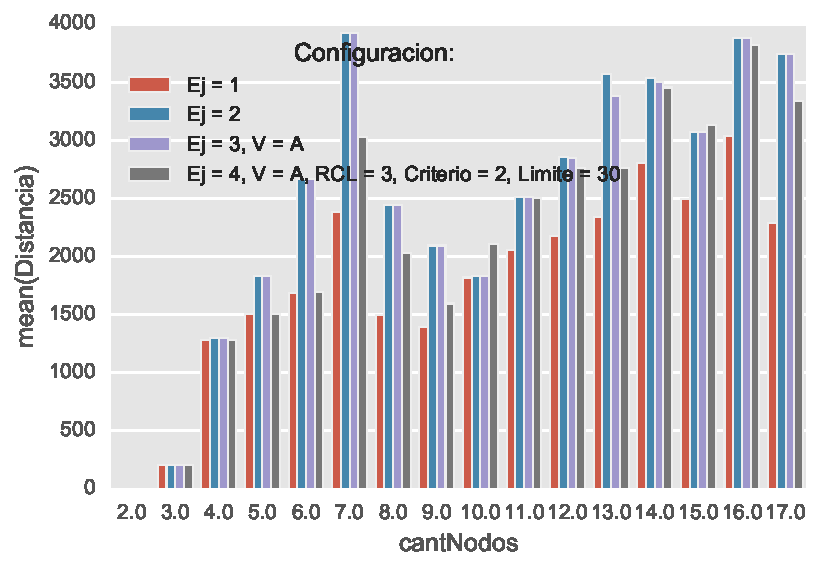
\includegraphics[\columnwidth]{imagenes/distancia_16_buena_distancia.pdf}
      \caption{}
    \end{center}
\end{figure}

      Como era de esperar, en general la implementación GRASP da mejores soluciones que las implementaciones golosa y de búsqueda local. En algunos casos tales como las instancias de 10 y 15 estaciones GRASP da una solución peor que los otros dos algoritmos heurísticos y esto puede deberse nuevamente a la aleatoriedad que contiene, tal como mencionamos anteriormente.

      \newpage

    \subsection{Experimento 2}
        Para este segundo experimento se compararon instancias de hasta 100 estaciones para dar una mejor idea del comportamiento de los algoritmos heurísticos comparándolos entre sí.

        En lo que respecta a tiempo de ejecución obtuvimos el siguiente gráfico basándonos en los resultados obtenidos:

\begin{figure}[H]
    \begin{center}
      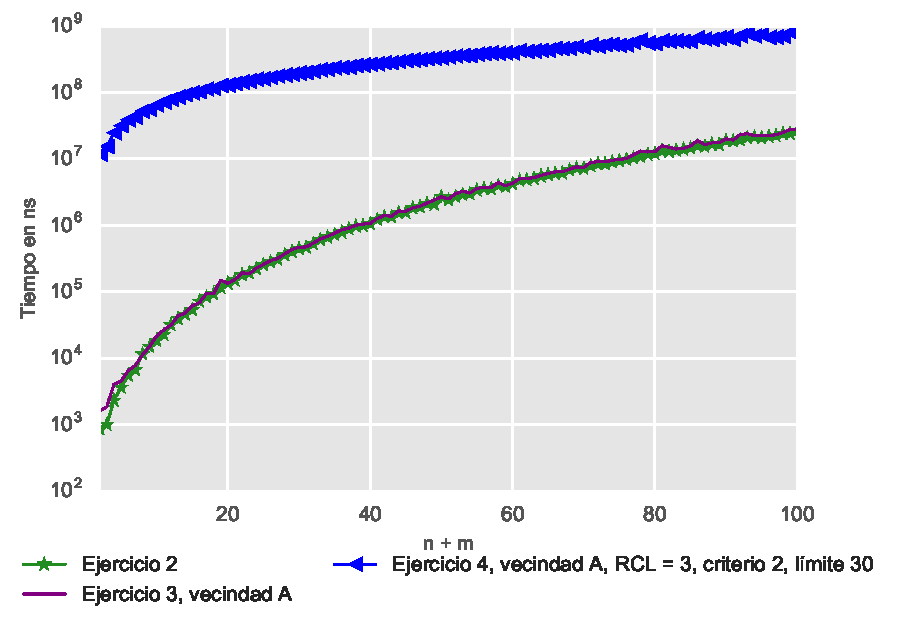
\includegraphics[\columnwidth]{imagenes/99_tiempo.pdf}
      \caption{}
    \end{center}
\end{figure}


        Al igual que en el gráfico del experimento anterior, el ejercicio 2 y 3 se mantienen casi a la par. Como podemos observar, confirmamos basándonos en nuestra hipótesis que ambos se mantienen lejanos (tiempo mucho menor) al ejercicio 4, pero veremos luego en el análisis de calidad de la solución cuán malo es esto, y además se acercan cada vez más a los tiempos de GRASP. Notemos como para 100 estaciones el ejercicio 4 toma casi un 99$\%$ más que los otros dos ejercicios, mientras que para instancias más chicas (20 estaciones) se acerca más a $99,9\%$ por lo que podemos entender que a instancias más grandes la diferencia de tiempo entre el ejercicio 4 y los ejercicios 2 y 3 sigue siendo amplia, pero se achica lentamente.

        Respecto a la calidad de la solución llegamos a construir el siguiente gráfico:

\begin{figure}[H]
    \begin{center}
      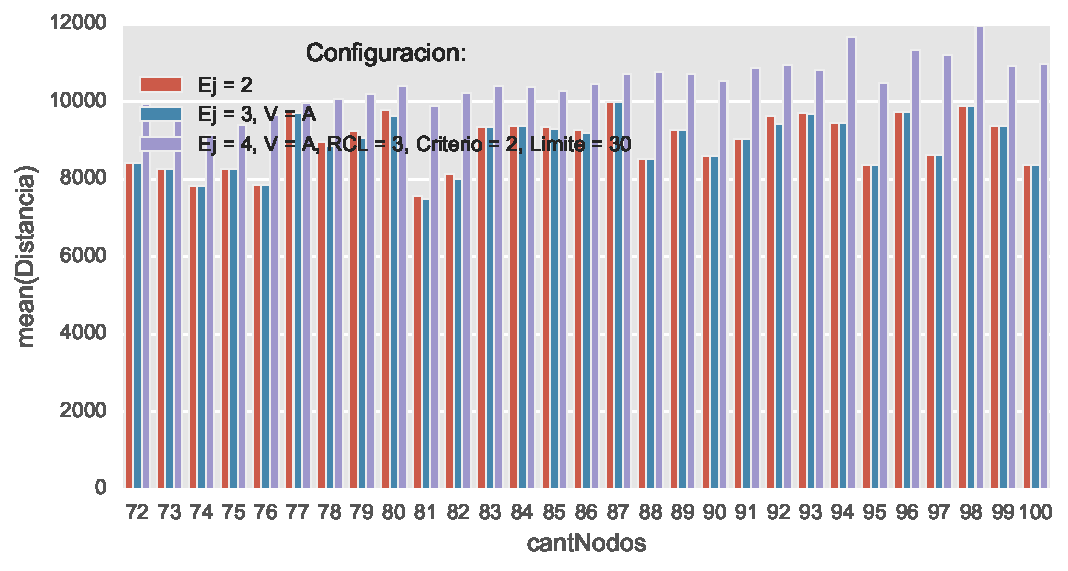
\includegraphics[width=1.08\columnwidth]{imagenes/99_distancia.pdf}
      \caption{}
    \end{center}
\end{figure}

        Luego de haber analizado los resultados de este último experimento nos llamó la atención ver que a diferencia del primer experimento, en este el ejercicio 4 se comportó de manera tal que las soluciones obtenidas con el mismo eran de aproximadamente hasta un $25\%$ peores que de los otros 2 ejercicios. También observamos que, con éxito en nuestra hipótesis, los resultados del ejercicio 3 se mantuvieron menores o iguales que las soluciones del ejercicio 2.

    \subsection{Conclusiones}
        Finalizando este informe, concluimos que si es necesaria una solución exacta para resolver nuestro problema entonces la única opción para asegurarnos la misma es utilizar la implementación de backtracking y esperar el tiempo que sea necesario, el cual no es mucho si son instancias de hasta 13 estaciones. En caso de que sea aceptable un posible error en la solución y no se espere siempre la óptima, es posible utilizar el algoritmo que realiza búsqueda local ya que la misma, como vimos, genera soluciones mejores o iguales que el algoritmo goloso.

        Dado que la implementación de GRASP tiene cierta aleatoriedad como vimos para instancias grandes no era la mejor implementación ni en tiempo ni en calidad de la solución por lo que no sería recomendable utilizar esta implementación para resolver este ejercicio salvo que se permita utilizar un RCL más grande y una cantidad de iteraciones mucho mayor, pero esto generaría un crecimiento en el tiempo de ejecución y tal vez termine siendo mejor utilizar backtracking ya que este no tiene configuraciones. Esto último se cumple particularmente para instancias chicas (no más de 13 estaciones) ya que para ese tipo de instancias backtracking supera en tiempo (es menor) al algoritmo de GRASP.